\documentclass[tikz,border=6pt]{standalone}
\usepackage{amsmath,amssymb,mathtools,physics,bm,nicefrac,wasysym}
\usepackage{xcolor}

\definecolor{colone}{RGB}{180,60,60}
\definecolor{coltwo}{RGB}{60,110,180}
\definecolor{colthree}{RGB}{60,140,80}

\definecolor{accent}{HTML}{A13D2C}
\definecolor{accent2}{HTML}{2B5F6B}
\definecolor{muted}{HTML}{5A564F}
\definecolor{panel}{HTML}{F8F6F0}
\definecolor{linecol}{HTML}{D8D2C4}
\definecolor{ink}{HTML}{1E1C1A}
\definecolor{astroblue}{HTML}{1B4F72}
\definecolor{astrodark}{HTML}{17202A}
\definecolor{sunyellow}{HTML}{E8A33D}

\usetikzlibrary{calc,arrows.meta,positioning,decorations.pathreplacing,decorations.markings,angles,quotes,shapes.geometric}
\usepackage{tikz-3dplot}

\newcommand{\vecr}{\vec r}
\newcommand{\vecL}{\vec L}
\newcommand{\vecA}{\vec A}
\newcommand{\vecf}{\vec f}
\newcommand{\vecF}{\vec F}
\newcommand{\vecp}{\vec p}
\newcommand{\avg}[1]{\left\langle #1\right\rangle}
\newcommand{\vecx}{\vec x}
\newcommand{\hatn}{\hat n}
\newcommand{\rhat}{\hat r}
\newcommand{\phihat}{\hat\phi}
\newcommand{\thetahat}{\hat\theta}
\newcommand{\note}[1]{\textcolor{blue!60!black}{\textit{[#1]}}}

% Astronomical acronyms
\newcommand{\LST}{\mathrm{LST}}
\newcommand{\GST}{\mathrm{GST}}
\newcommand{\GMST}{\mathrm{GMST}}
\newcommand{\GAST}{\mathrm{GAST}}
\newcommand{\LMST}{\mathrm{LMST}}
\newcommand{\LAST}{\mathrm{LAST}}
\newcommand{\UT}{\mathrm{UT}}
\newcommand{\UTC}{\mathrm{UTC}}
\newcommand{\TAI}{\mathrm{TAI}}
\newcommand{\TT}{\mathrm{TT}}
\newcommand{\TDB}{\mathrm{TDB}}
\newcommand{\JD}{\mathrm{JD}}
\newcommand{\MJD}{\mathrm{MJD}}
\newcommand{\EoT}{\mathrm{EoT}}
\newcommand{\SNR}{\mathrm{SNR}}
\newcommand{\RON}{\mathrm{RON}}

% Helper commands for specific diagrams
\newcommand{\midlinelabel}[3]{
    \node (midlabel) at ($ (#1)!.5!(#2) $) {#3};
    \draw[stealth-] (#1) --  (midlabel);
    \draw[-stealth] (midlabel) -- (#2);
}
\newcommand{\midlinelabell}[3]{
    \node[fill = white, inner sep = 0.2pt, outer sep=3pt] (midlabel) at ($ (#1)!.5!(#2) $) {#3};
    \draw[stealth-] (#1) --  (midlabel);
    \draw[-stealth] (midlabel) -- (#2);
}
\newcommand{\midlinelabelll}[3]{
    \node[fill = white, inner sep = 0.2pt, outer sep=3pt,scale=0.6] (midlabel) at ($ (#1)!.5!(#2) $) {#3};
    \draw[stealth-] (#1) --  (midlabel);
    \draw[-stealth] (midlabel) -- (#2);
}



\begin{document}
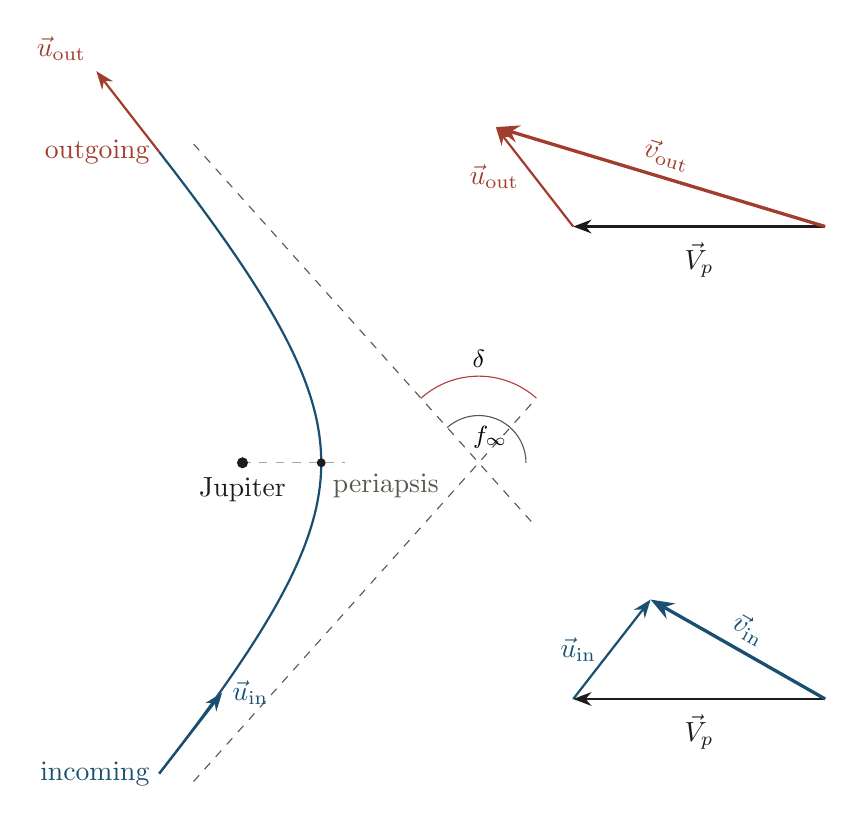
\begin{tikzpicture}[>=Stealth, scale=1.0, font=\normalsize]

		% ---------- Shared geometry, computed once at top level so both
		% panels can reference the same numbers (a TikZ scope is a TeX
		% group, so macros set inside one scope are not visible in another)
		\def\ecc{1.5}
		\def\lsr{2.5}
		\def\cut{105}
		\pgfmathsetmacro{\finf}{acos(-1/\ecc)}   % 131.81 deg
		\pgfmathsetmacro{\vin}{180-\finf}         % 48.19 deg
		\pgfmathsetmacro{\aa}{\lsr/(\ecc*\ecc-1)}
		\pgfmathsetmacro{\cc}{\aa*\ecc}

		% True local tangent directions at the curve's own endpoints (not
		% the infinite-limit angle, which the curve has not fully reached
		% yet at this finite truncation): with r(v)=lsr/(1+e cos v),
		% dr/dv = e sin(v) r(v)^2/lsr, and the tangent direction is
		% atan2(dy/dv, dx/dv) with x=r cos v, y=r sin v
		\pgfmathsetmacro{\rcut}{\lsr/(1+\ecc*cos(\cut))}
		\pgfmathsetmacro{\rpout}{\ecc*sin(\cut)*\rcut*\rcut/\lsr}
		\pgfmathsetmacro{\dxout}{\rpout*cos(\cut)-\rcut*sin(\cut)}
		\pgfmathsetmacro{\dyout}{\rpout*sin(\cut)+\rcut*cos(\cut)}
		\pgfmathsetmacro{\tangout}{atan2(\dyout,\dxout)}
		\pgfmathsetmacro{\rpin}{\ecc*sin(-\cut)*\rcut*\rcut/\lsr}
		\pgfmathsetmacro{\dxin}{\rpin*cos(-\cut)-\rcut*sin(-\cut)}
		\pgfmathsetmacro{\dyin}{\rpin*sin(-\cut)+\rcut*cos(-\cut)}
		\pgfmathsetmacro{\tangin}{atan2(\dyin,\dxin)}

		% ================= Panel A: hyperbolic geometry in Jupiter's frame =================
		% NOTE: drawn with a schematic eccentricity (ecc=1.5, not the
		% problem's e=1.2) purely so the asymptotes cross visibly close to
		% the curve; no numeric angle values are printed in this panel,
		% only the symbols delta and f_infty, so this substitution
		% introduces no inconsistency -- the actual numbers are computed
		% from the real e=1.2 in the text below.
		\begin{scope}
			\coordinate (O) at (0,0);
			\coordinate (Ctr) at (\cc,0);

			% Literal asymptotes: two lines through the center, parallel to
			% the focus's own asymptotic radius directions (+f_infty,
			% -f_infty), each drawn over a finite stretch that hugs the
			% curve closely
			\draw[muted, dashed] ($(Ctr)+({-1*cos(\finf)},{-1*sin(\finf)})$) -- ($(Ctr)+({5.5*cos(\finf)},{5.5*sin(\finf)})$);
			\draw[muted, dashed] ($(Ctr)+({-1*cos(-\finf)},{-1*sin(-\finf)})$) -- ($(Ctr)+({5.5*cos(-\finf)},{5.5*sin(-\finf)})$);

			% Hyperbola branch, exact polar form r = lsr/(1+e cos v)
			\draw[astroblue, thick, domain=-\cut:\cut, samples=120, smooth, variable=\v]
				plot ({(\lsr/(1+\ecc*cos(\v)))*cos(\v)}, {(\lsr/(1+\ecc*cos(\v)))*sin(\v)});

			% Periapsis axis (short reference line) and point
			\draw[ink!40, dashed] (O) -- (1.3,0);
			\fill[ink] ({\lsr/(1+\ecc)},0) circle (1.6pt);

			% Focus
			\fill[ink] (O) circle (2pt) node[below=2pt] {Jupiter};

			% Reference points for the angle pics (named coordinates only;
			% the angles library cannot parse inline calc expressions as
			% pic vertices). These use the exact, infinite-limit asymptotic
			% directions (vin, f_infty), since delta and f_infty are
			% defined as limits at r->infty, and are marked at the actual
			% asymptote crossing point, Ctr.
			\coordinate (Pref) at ($(Ctr)+(1,0)$);
			\coordinate (Uin) at ($(Ctr)+({cos(\vin)},{sin(\vin)})$);
			\coordinate (Uout) at ($(Ctr)+({cos(\finf)},{sin(\finf)})$);

			\coordinate (Pin) at ({\rcut*cos(-\cut)},{\rcut*sin(-\cut)});
			\coordinate (Pout) at ({\rcut*cos(\cut)},{\rcut*sin(\cut)});

			% Velocity-direction arrows, drawn tangent to the curve at its
			% own endpoints (true local tangent, not the infinite-limit
			% direction)
			\draw[->, astroblue, thick] (Pin) -- ($(Pin)+({1.3*cos(\tangin)},{1.3*sin(\tangin)})$) node[right] {$\vec u_{\rm in}$};
			\draw[->, accent, thick] (Pout) -- ($(Pout)+({1.3*cos(\tangout)},{1.3*sin(\tangout)})$) node[above left] {$\vec u_{\rm out}$};

			% delta and f_infty, both marked at Ctr, the asymptotes' actual
			% crossing point
			\draw pic["\small $\delta$", draw=colone, angle radius=11mm, angle eccentricity=1.2]
				{angle=Uin--Ctr--Uout};
			\draw pic["\small $f_\infty$", draw=muted, angle radius=6mm]
				{angle=Pref--Ctr--Uout};

			\node[muted, below right=1pt] at ({\lsr/(1+\ecc)},0) {periapsis};
			\node[astroblue, left] at (Pin) {incoming};
			\node[accent, left] at (Pout) {outgoing};
		\end{scope}

		% ================= Panel B: heliocentric vector addition, two separate diagrams =================
		% V_p points left; u_in/u_out are parallel-transported copies of
		% the EXACT SAME vectors drawn in Panel A (same tangout/tangin
		% angles, same length), attached tip-to-tail at V_p's arrowhead.
		\def\Vp{3.2}
		\def\uu{1.6}

		% Diagram 2: V_p + u_out (long resultant)
		\begin{scope}[xshift=7.4cm, yshift=3.0cm]
			\coordinate (O) at (0,0);
			\coordinate (A) at (-\Vp,0);
			\coordinate (Bout) at ($(A)+({\uu*cos(\tangout)},{\uu*sin(\tangout)})$);

			\draw[->, ink, thick] (O) -- (A) node[pos=0.5, below=2pt] {$\vec V_p$};
			\draw[->, accent, thick] (A) -- (Bout) node[pos=0.5, left=2pt] {$\vec u_{\rm out}$};
			\draw[->, accent, very thick] (O) -- (Bout) node[pos=0.5, sloped, above] {$\vec v_{\rm out}$};
		\end{scope}

		% Diagram 1: V_p + u_in (short resultant)
		\begin{scope}[xshift=7.4cm, yshift=-3.0cm]
			\coordinate (O) at (0,0);
			\coordinate (A) at (-\Vp,0);
			\coordinate (Bin) at ($(A)+({\uu*cos(\tangin)},{\uu*sin(\tangin)})$);

			\draw[->, ink, thick] (O) -- (A) node[pos=0.5, below=2pt] {$\vec V_p$};
			\draw[->, astroblue, thick] (A) -- (Bin) node[pos=0.5, left=2pt] {$\vec u_{\rm in}$};
			\draw[->, astroblue, very thick] (O) -- (Bin) node[pos=0.5, sloped, above] {$\vec v_{\rm in}$};
		\end{scope}
	\end{tikzpicture}
\end{document}
